% -*- latex -*-
%-----------------------------------------------------------------------
%;  Copyright (C) 2003
%;  Associated Universities, Inc. Washington DC, USA.
%;
%;  This program is free software; you can redistribute it and/or
%;  modify it under the terms of the GNU General Public License as
%;  published by the Free Software Foundation; either version 2 of
%;  the License, or (at your option) any later version.
%;
%;  This program is distributed in the hope that it will be useful,
%;  but WITHOUT ANY WARRANTY; without even the implied warranty of
%;  MERCHANTABILITY or FITNESS FOR A PARTICULAR PURPOSE.  See the
%;  GNU General Public License for more details.
%;
%;  You should have received a copy of the GNU General Public
%;  License along with this program; if not, write to the Free
%;  Software Foundation, Inc., 675 Massachusetts Ave, Cambridge,
%;  MA 02139, USA.
%;
%;  Correspondence concerning AIPS should be addressed as follows:
%;          Internet email: aipsmail@nrao.edu.
%;          Postal address: AIPS Project Office
%;                          National Radio Astronomy Observatory
%;                          520 Edgemont Road
%;                          Charlottesville, VA 22903-2475 USA
%-----------------------------------------------------------------------
%Body of intermediate AIPSletter for 31 December 2003

\documentclass[twoside]{article}
\usepackage{graphics}

\newcommand{\AIPRELEASE}{June 30, 2003}
\newcommand{\AIPVOLUME}{Volume XXIII}
\newcommand{\AIPNUMBER}{Number 1}
\newcommand{\RELEASENAME}{{\tt 31DEC03}}
\newcommand{\NEWNAME}{{\tt 31DEC03}}
\newcommand{\OLDNAME}{{\tt 31DEC02}}

%macros and title page format for the \AIPS\ letter.
\input LET98.MAC
%\input psfig

\newcommand{\MYSpace}{-11pt}

\normalstyle

\section{General developments in \AIPS}

\subsection{Linux news: bad and better compilers}

Instructions for fetching and installing the GNU 2.95.3 compiler are
given on the \AIPS\ web page.  The tar file is directly available from
NRAO\@.  This is needed since the 2.96.x compiler, shipped with some
versions of Linux, does not optimize code properly.  Users of more
recent Linux versions, \eg\ RedHat 9, will probably want to use the
GNU 3.3 compiler which comes with it.  Setting {\tt OPT2} simply to
{\tt ``-O2''} in {\tt \$SYSLOCAL/FDEFAULT.SH}, produces code as fast
on the {\tt DDT test} as 2.95.3 with its complex {\tt OPT2}\@.  On the
larger {\tt Y2K} test, 3.3 is about 5\%\ slower in real time and 13\%\
slower in cpu on a RedHat 7.2, Pentium IV 1.3 GHz computer.  The
2.95.3 libraries are very dated compared to the more recent operating
systems, suggesting that it is finally time to update despite the
modest loss in performance.

\subsection{Current and future releases}

We now have formal \AIPS\ releases on an annual basis with binary
releases only for Solaris and Linux.  All architectures can do a full
installation from the source files.  The next release is called
\RELEASENAME\ and remains under active development.  You may fetch and
install a complete copy of this version at any time.  This
\Aipsletter\ is intended to advise you of developments to date in this
new release.  Having fetched \RELEASENAME, you may update your
installation whenever you want by running the so-called ``Midnight
Job'' (MNJ) which uses transaction files to copy and compile the code
selectively based on the code changes and compilations we have done.
We expect users to take the source-only version of {\tt 31DEC03}
\AIPS\ over the Internet (via \emph{anonymous} ftp); there is a guide
to the install script and an \AIPS\ Manager FAQ page on the \AIPS\ web
site.

The MNJ has been changed.  It now serves up \AIPS\ incrementally using
the Unix tool {\tt cvs} running with anonymous ftp.  Linux sites will
almost certainly have {\tt cvs} installed; other sites may have
installed it along with other GNU tools.  Secondary MNJs will still be
possible using {\tt ssh} or {\tt rcp} or NFS as with previous
releases.  We have found that {\tt cvs} works very well, although it
has one quirk.  If a site modifies a file locally but in an
\AIPS-standard directory, {\tt cvs} will detect the modification and
attempt to reconcile the local version with the NRAO-supplied version.
This usually produces a file that will not compile or run as intended.

\AIPS\ is now copyright \copyright\ 1995 through 2003 by Associated
Universities, Inc., NRAO's parent corporation, but may be made freely
available under the terms of the Free Software Foundation's General
Public License (GPL)\@.  This means that User Agreements are no longer
required, that \AIPS\ may be obtained via anonymous ftp without
contacting NRAO, and that the software may be redistributed (and/or
modified), under certain conditions.  The full text of the GPL can be
found in the \texttt{15JUL95} \Aipsletter.

\section{Patch Distribution for \OLDNAME}

As before, important bug fixes and selected improvements in
\OLDNAME\ can be downloaded via the Web beginning at:

\begin{center}
\vskip -10pt
{\tt http://www.aoc.nrao.edu/aips/patch.html}
\vskip -10pt
\end{center}

Alternatively one can use {\it anonymous} \ftp\ to the NRAO server
{\tt ftp.aoc.nrao.edu}.  Documentation about patches to a release is
placed on this site at {\tt pub/software/aips/}{\it release-name} and
the code is placed in suitable subdirectories below this.  As bugs in
\NEWNAME\ are found, they are simply corrected since \NEWNAME\ remains
under development.  Corrections and additions are made with a midnight
job rather than with manual patches.  Remember, no matter when you
received your copy of \OLDNAME\ {\it you must} fetch and install its
patches if you require them.

The \OLDNAME\ release had a few important patches including new ones
in June.  These were:
\begin{enumerate}
\item\ {\tt KNTR} to handle {\tt LTYPE} not 3 for polarization vectors
       {\it 2003-01-03}.
\item\ {\tt FITLD} to handle multiple data types in one tape {\it
       2003-01-03}.
\item\ {\tt IRING} to correct the centering {\it 2003-01-10}.
\item\ {\tt LWPLA} to use {\tt ASPMM} for new {\tt GREYS}, {\tt KNTR},
       {\tt PCNTR} plots {\it 2003-01-16}.
\item\ {\tt FILLM} and {\tt PRTTP} to read short records in VLA
       archive disk files {\it 2003-03-20}.
\item\ {\tt INDXR} to fill VLBI {\tt CL} table properly {\it
       2003-05-21}.
\item\ RedHat 9 to link edit requires fixed Z routines {\it
       2003-06-24}.
\item\ {\tt SETFC} to format field numbers $> 999$ correctly {\it
       2003-06-27}.
\end{enumerate}

\section{Recent \AIPS\ and related Memoranda}

The following new \AIPS\ Memorandum is available from the \AIPS\ home
page.

\begin{tabular}{lp{5.8in}}
108 &  Weights for VLA Data \\
   &   Bryan J. Butler (NRAO)\\
   &   January 21, 2003\\
   &   A method for calculating the properly calibrated weights for
VLA data in \AIPS\ (or AIPS++, or any other package) is presented,
along with some related information on the ``nominal sensitivity''
quantity stored in the VLA archive data.  A method of determining the
quantity $T_{sys} / \eta_a$ for each antenna using the properly
calibrated weights is also presented.
\end{tabular}

\section{\AIPS\ Distribution}

We are now able to log apparent MNJ accesses and recently acquired a
tool to log downloads of the tar balls.  The software that managed the
registration database is broken and appeals to have it fixed have
fallen on deaf ears.  There appear to be about 71 sites/machines that
have run the MNJ on {\tt 31DEC03} at least occasionally.  In the
period May 19 --- July 1, there have been downloads to 30 sites of
the {\tt 31DEC02} tar ball and downloads to 91 sites of the {\tt
31DEC03} tar ball.  This is at a rate of 0.7 and 2.0 download sites
per day.
\vfill\eject

\section{Improvements of interest to users in \RELEASENAME}

We expect to continue publishing the  \Aipsletter\ approximately every
six months along with the annual releases.  There have been a number
of changes in \RELEASENAME.  A package of \AIPS\ procedures, called
{\tt VLARUN}, to reduce VLA data in a pipeline, similar to the one in
use for VLBA data, was added.  Two experimental display tasks were
created; {\tt SCLIM} scales images to be used as inputs to {\tt LAYER}
which creates a colored image ``layering'' up to 10 input images.  The
new task {\tt SHADO} determines the loss in sensitivity due to
shadowing for prospective array designs.  New task {\tt DQUAL} gets
rid of all qualifier numbers on sources in a \uv-data file.  The new
verb {\tt IMDIST} determines the angular distance between two image
pixels and new procedure {\tt TVDIST} uses the TV to select the two
pixels for {\tt IMDIST}\@.  New verb {\tt IM2TV} converts image pixel
to TV pixel coordinates, while new verb {\tt TVILINE} draws a line on
the TV between two image pixels.

\AIPS\ has been ported to the Apple MacIntosh OS/X operating system
and its use on the latest RedHat (version 9) has been established.
The Mac performance needs to be improved, but awaits compiler studies.

Other than relatively minor differences, \RELEASENAME\ is compatible
in all major ways with the with the {\tt 15OCT98} and later releases.
There are significant incompatibilities with older versions.

\subsection{UV data calibration}

\subsubsection{CLCAL, SNSMO, CLSMO}

The subject of the smoothing of calibration tables received
significant attention.  The calibration routines depended on flagging
records in {\tt SN} and {\tt CL} tables and then adding new records.
The routine that re-references phases for {\tt CLCAL} and {\tt CALIB}
was found to ignore the flagging of records, restoring them to full
status.  {\tt SNSMO} also had this problem.  They were fixed, but, to
avoid similar problems elsewhere, {\tt CALSEL} (used in {\tt CLCAL},
{\tt CALIB}, {\tt FRING} and {\tt KRING}) was changed so that tables
are re-written with no flagged records.  The smoothing routines
previously used went to great lengths to return values at all times,
even if the times were very distant from any valid data.  They were
replaced with a wider variety of functions that strictly honor a
support size and return blanked values when appropriate.  The new
routines offer the choice of smoothing data from different sources
together or keeping them separate.  They also understand about blanked
values; some of the earlier functions did not.

Tasks {\tt SNSMO} and {\tt CLSMO} were changed to smooth larger data
sets, to offer the new smoothing functions, to set the support size
and function parameters, to control smoothing between sources, and to
control what data in the tables are replaced by the smoothed values.
The last has already been a source of user confusion: if {\tt DOBLANK}
$\ge 0$, then previously blanked solutions are replaced by smoothed
values and if {\tt DOBLANK} $\le 0$, then previously good solutions
are replaced by smoothed solutions.  Thus the user can choose to keep
or replace failed solutions and can choose to smooth the good data or
not.

{\tt CLCAL} suffered from an attempt to combine operations involving
the smoothing of the merged {\tt SN} table with operations applying
that smoothed table to the {\tt CL} table.  These operations are now
specified with a variety of additional adverbs.  The smoothing is
controlled by the adverbs also used in {\tt SNSMO}.  The default {\tt
CL} table versions have been changed and, if {\tt GAINUSE = 0}, the
input {\tt CL} table is copied as a whole to the new output table
before the interpolation operations.  Smoothing for phase now uses the
real and imaginary parts rather than a somewhat modified smoothing of
actual phases.  {\tt CLCAL} was given the option to do its things for
a range of {\tt SN} table versions, rather than using only one or all.
The {\tt 'SMOO'} operation was dropped --- {\tt 'MERG'} will do fine
with the separated smoothing control adverbs.  The use of {\tt CLCAL}
for single-source files was corrected.  Previously it had odd bits
that seemed to limit it to a single input {\tt SN} table with no
smoothing.

\subsubsection{VLARUN}

{\tt VLARUN} is a {\tt RUN} file that consists of a collection of
procedures allowing straightforward calibration and simple imaging of
continuum and spectral-line VLA data.  It is particularly useful for a
quick look, \eg\ to decide whether particular VLA archive data are
useful for the intended science without spending too much time
calibrating and imaging.  It will apply the calibration scheme as
outlined in Appendix D of the AIPS Cookbook, \ie\ it will calibrate
the visibility phase first which makes it suitable for high-frequency
data as well.

{\tt VLARUN} assumes that flagging has been performed.  If flagging in
the line data is needed, it is assumed that these flags are copied to
the ``channel-0'' file flag table before {\tt VLARUN} is started.
Furthermore, only a single frequency ID should be present in the
file(s).  The observations must include at least one of the default
VLA flux calibrators (as known by {\tt SETJY}); for other flux
calibrators a simple edit of the procedure is necessary.

The procedure will automatically calibrate the continuum or
`'channel-0'' and line part of a spectral-line data set. At several
stages during the process, {\tt VLARUN} creates plot files which can
be viewed to assess the calibration.  The user may also opt to perform
simple imaging, \eg\ to obtain a first model of the targeted sources
for self-calibration.

Current practice suggests calibrating the data, assessing the
calibration, and including additional flagging in flag table number
one.  Then re-run the procedures.  Note that for scientific purposes,
it is assumed that the user will flag and re-image the data properly
instead of using {\tt VLARUN}'s output.

\subsubsection{Other matters}

\begin{description}
\myitem{CLCOR} now has a new {\tt OPCODE=`ATMO`}\@.  Using an input
               text file, this option corrects the data for excess
               zenith path delays.
\myitem{TECOR} was corrected to handle a change in the format of {\tt
               IONEX} input files.
\myitem{LOCIT} is now in production use finding antenna locations at
               the VLA\@.  As a consequence, bugs revealed by odd
               circumstances in the data were found and fixed.
\myitem{EDITR} tried to avoid extra work too much and so failed to
               flag data under some crowded circumstances.  The task
               now copies the input {\tt FG} table to a new one and
               adds the new flags to that version.
\myitem{WIPER} was given defenses against bad windows and the {\tt
               DOCENTER} option to control placement of the menu.
\end{description}

\subsection{UV data handling}

\subsubsection{FILLM}

{\tt FILLM} received considerable attention over the last few months.
Its disk reading handled the case in which there were short physical
records in a logical so long as the first physical record was not
short.  But the first (and only) physical record in a logical can
easily be short (continuum with $< 26$ antennas in the sub-array), so
the reading could get off and find no more data.  The signal was a
read error at the end with fewer than 13*2048 bytes, but ``error
code'' 0. The last physical record could also be short, which required
smarter ``error'' handling to report only real errors.  {\tt PRTTP}
was also corrected for these issues.  The channel 0 frequency
increment was corrected.

{\tt FILLM}, at the VLA and AOC,  is able to load data to \AIPS\ as it
is observed.  This on-line {\tt FILLM} has depended on a second
process to be running to read the data from the VLA and pass it on as
if it were the tape device.  For a variety of reasons, including when
the VLA ModComps would go down, this process would disappear and the
on-line {\tt FILLM} would quit or be left sitting there not getting
any data.  The second process was revised to make it more robust and
various re-try methods were added to the on-line portion of the {\tt
FILLM} tape routines.  After that, on-line {\tt FILLM} ran for over a
week surviving a 2-day shutdown and numerous other ``irregularities.''
During this period a new plan was devised which will probably soon be
put in place.  Under this plan, the archive data will be written to
disk at the VLA and to a mirror disk in the AOC\@.  A new file will be
written each day.  Then on-line {\tt FILLM} will simply read the
current day's disk file and, when it reaches the end-of-file, it will
go into a special mode to read data as they are added to the file and
even to switch to the next day's file when appropriate.

New options were also added to {\tt FILLM}\@.  An option to use the
data weighting described in \AIPS\ Memo 108 was added ({\tt DOWEIGHT =
10}\@.  This weighting has a better scaling than that present in {\tt
FILLM} since 2000.  Another new option was added to choose to omit
visibilities for which one of the antennas failed its last reference
pointing attempt (bit 10 of {\tt CPARM(2)}).  The default is to do as
it does now --- load all the data --- but then it makes an {\tt OF}
table which holds the reference pointing information along with the
antenna shadowed bit.  We should construct a task to use this table
for editing.

\subsubsection{Other matters}

\begin{description}
\myitem{UVFIX} was revised to do multi-source files (with no position
               shifting), to recognize GMRT data with its different
               sign convention (they believed \AIPS' documentation!),
               to do a more accurate phase shift on position shifts,
               and to make a more consistent interpretation of the
               data epoch and array identity.
\myitem{DBCON} did correct phase shifts only for rather small position
               shifts.  It has been corrected to do full-accuracy
               phase shifts and to recompute $(u,v,w)$ for the new
               reference coordinate.
\myitem{INDXR} failed to initialize VLA {\tt CL} tables correctly when
               the weather table was not being used, such as when the
               user specifies the opacity or only wants antenna gain
               corrections.  Similarly, it failed to initialize VLBA
               {\tt CL} tables with data from the {\tt IM} and {\tt
               MC} tables under most cases.  This initialization used
               the dispersive delay from the {\tt IM} table.  That is
               now blocked since \AIPS\ applies the dispersive delay
               in calibration and the delay in the {\tt IM} table has
               already been applied.  A similar blocking was added to
               {\tt FITLD}\@.  This has not mattered since the
               dispersive delays seem always to be zero in the {\tt
               IM} tables.
\myitem{UVCOP} was changed to copy all sources to the {\tt SU} table
               since it copies all references to sources in {\tt CL}
               tables.  {\tt CLCOR} had trouble with missing sources
               otherwise.  Flagging was not done when the flag table
               entry specified the {\tt FQ} number, but all {\tt FQ}s
               were being copied.
\myitem{LISTR} was corrected to average phases always with vector
               methods; it previously scalar-averaged phases
               literally.  Changed the display of the {\tt MATX}
               average to include the vector average of all the data
               as well as the literal average of the printed values
               given previously.  Fixed the formating for flagged gain
               solutions.
\myitem{weights} assigned to combination polarizations, \eg\ Ipol, were
               incorrectly computed as the simple average of weights.  The
               correct weights have been implemented using the real
               formula.
\myitem{DQUAL} is a new task to remove all qualifiers from a source
               table, renumbering the sources in the \uv\ data and
               source table.
\end{description}

\subsection{Data display and analysis}

\subsubsection{SCLIM and LAYER}

{\tt SCLIM} is a new task which creates images scaled from 0 to 1
using corners, function types, pix-ranges, etc.  Clipped values ---
even at the top --- may be set to 0 on output.  It was written to
create inputs to the new and experimental task {\tt LAYER}\@.  That
task reads as many as 10 images letting each ``absorb'' the current
image and add to that image by emission with optical depths scaled from
the input image values, all optionally colored.  This will be tricky
to use, but good results should be possible.

\subsubsection{Other matters}

\begin{description}
\myitem{MOMNT} was overhauled to handle blanked pixels correctly.
               Smoothing with zeros is not correct and {\tt MOMNT} did
               not even check for magic blanks.  Buffer sizes were
               raised.  The option to adjust the cutoff level for the
               primary beam was added.  This allows {\tt MOMNT} to
               work on the output of {\tt PBCOR} which is required
               since the primary beam is a function of frequency.  a
               bug affecting the history file was corrected.
\myitem{IMDIST} is a new verb to compute the spherical distance
               between two pixels in two images.  {\tt TVDIST} is a
               new procedure to read two pixels from the TV and then
               invoke {\tt IMDIST} on them.
\myitem{IM2TV} is a new verb to convert an image pixel coordinate to a
               TV coordinate.
\myitem{TVILINE} is a new verb to draw a line on the TV between to
               image pixel coordinates.  ({\tt TVLINE} uses TV
               coordinates.)
\myitem{IMVAL} as well as {\tt QIMVAL}. {\tt MAXFIT}, {\tt TVFLUX} and
               {\tt TVMAXFIT} now return {\tt COORDINA} as an output
               adverb.
\myitem{IMEAN} and {\tt IMSTAT} can return the statistics of a
               circular aperture in an image as well as a rectangular
               one.
\myitem{plots} on the TV that have waited for 30 seconds before
               showing a new page may now be held indefinitely by
               pressing button A, while B and C go on immediately, and
               D exits.
\myitem{POSSM} had a variety of bugs fixed including one that could
               hang {\tt AIPS} itself.  Bugs triggered by missing data
               in multiple plots, by plotting amplitudes, and by
               position shifting were corrected.
\myitem{TVCPS} now has the CMYK (printer colors) option in addition to
               the usual RGB\@.  Different gamma corrections must be
               used for the two color schemes.
\myitem{LWPLA} now allows for gamma corrections so that the needs of
               RGB, CMYK, and various printers may be addressed.  The
               scaling options ({\tt DPARM}s) were made more
               intuitive.
\myitem{PLCUB} now has an option to omit the frame axis labeling
               entirely.
\myitem{TVRGB} has new adverbs to control separately the sub-image for
               the interactive TV portion and the sub-image to be
               written out at the end.  The limitation to the maximum
               TV size has been eliminated along with bugs handling
               {\tt TXINC} and {\tt TYINC}\@.
\myitem{TVHUI} also had its adverbs changed and bugs fixed in scaling
               the hue and saturation images and reporting the final
               pix-ranges.
\end{description}

\subsection{Imaging and miscellaneous}

\begin{description}
\myitem{IMAGR} had only a few changes.  It defends itself now against
               bad {\tt BOX} values.  It writes out the peak residual
               left in each field to its history file.  It allows
               beams for Cleaning to be made up to 16384 on a side if
               {\tt IMAGRPRM(10)} is actually set suitably.
\myitem{WISH} survey data (southern Westerbork, -25 to -15 or -9
               degrees declination) have been inserted into the WENSS
               source lists used in imaging interfering sources.
\myitem{SETFC} was corrected to use a suitable format for facet
               numbers $> 999$.
\myitem{TASAV} now copies all extension files (including plot files)
               for images as well as \uv-data files.
\myitem{output} adverbs from verbs and tasks are now viewed with the
               verb {\tt OUTPUTS} rather than {\tt INPUTS}\@.
\end{description}

\subsection{Array and data modeling}

\begin{description}
\myitem{CONFI} was revised substantially.  The topography file may now
               be in free format.  The definition of worst side-lobe
               was changed as well as the technique for finding it.
               This allows some optimization of the main lobe shape.
               The gain in the optimization loop was made adaptive
               under user control.  Bugs affecting or caused by user
               input were corrected or prevented.
\myitem{SHADO} is a new task to estimate the loss of sensitivity due
               to shadowing of the antennas by each other.
\myitem{UVSIM} was changed to use true IAT times when possible, \ie\
               when the user provides the array location.  The
               observing date and coordinates were changed to 2000
               from 1950.  This allows {\tt UVFIX} to be run on the
               output file.
\myitem{UVCON} was also changed to compute correct IAT times, allowing
               {\tt UVFIX} to work on the data.  Random antenna-based
               phase and amplitude errors may be added to the data.
\end{description}

\section{Improvements of interest to \AIPS\ managers in \RELEASENAME}

\subsection{MacIntosh OS/X}

\AIPS\ now works on Apple MacIntosh systems running the OS/X operating
system.  Details of how to prepare a Mac to install \AIPS\ are given
on a page of the main \AIPS\ web page.  Basically, one has to acquire
a C compiler, a Fortran compiler, and X Windows.  The port was
relatively simple.  One of the major ``gotchas'' was the fact that
OS/X is case insensitive at some, but not all, times.  Thus, \AIPS\
procedures {\tt AS}, {\tt GREP}, {\tt PWD}, and {\tt WHICH} had to be
renamed by prepending {\tt AI} to the name.  Numerous procedures had
to have references to these (primarily {\tt PWD}) corrected.
Architecture case statements required addition of the {\tt MACPPC}
architecture.  The Mac uses Z routines in {\tt \$APLMAC}, then {\tt
\$APLLINUX}, and so forth up the tree.  There are only a few Z
routines in the Mac area, including stubbed routines for magnetic
tapes.

The performance achieved was less than was hoped.  An 800 MHz iBook
laptop (the G3 chip) achieved an \AMark\ of 18.  For comparison, a 1
GHz Intel laptop is about 40.  When \AIPS\ was then installed on a
800 MHz PowerBook laptop (G4 chip), the performance was identical!
For the moment, we are unable to get the {\tt g77} compiler to
optimize properly for Macs, especially the powerful G4 chip.  GNU is
making progress on their compiler; the latest will at least {\tt make}
on Macs, but the optimization so far fails.  Wes Young is looking into
this for us.

\subsection{install.pl}

The installation script {\tt install.pl} was modified in a number of
ways in the past six months.  An error in dealing with the question
about unpacking the tar ball was corrected.  The page about TV sockets
was removed; it confused people and did nothing.  For the Mac port, it
was corrected to use {\tt AIPWD} rather than {\tt PWD}, to recognize
the {\tt MACPPC} architecture, and to look for {\tt readline} in the
usual place on Macs.  For installations on systems already having an
\AIPS, it now renames the {\tt TEXT} directory before starting.
Otherwise, the load of that directory failed.  The MNJ corrected this
but at considerable expense.  Registration no longer works, so it was
commented out of the script.  The default {\tt \$AIPS\_ROOT} was moved
to the current directory.

\subsection{Other matters}

\begin{description}
\myitem{startup} procedures were changed to get the host name by
                 calling new scripts {\tt SETNAME} and {\tt SETUNAME}.
                 The main use is for laptop computers since they often
                 get a new name every time they connect to the LAN\@.
                 The {\tt LOGIN} files may set the variable {\tt
                 LAPTOP} to {\tt YES} in this case.
\myitem{RedHat 9} forced a few changes to Z routines.  These were in
                 the nature of removing direct references to system
                 {\tt external} variables such as {\tt errno}.  They
                 are replaced with includes or subroutine calls.
\myitem{ZLPCL2} was changed to work with the {\tt ghostview}
                 previewer to convert print files to PostScript and
                 then display them correctly.
\myitem{FDEFAULT} \hspace{1em} was changed for Linux to specify the
                 correct {\tt OPT2} option for GNU 3.2+ compilers.
                 The older 2.95.3 options are present but commented
                 out; 2.95.3 will also work with the new option.
\end{description}


\section{Preview of coming attractions}

Subtle colors used to indicate polarization vector angles, channel
number in contouring, IF number, etc.

Multiple overlapping solution intervals

Corrections for atmospheric delay and the troposphere

Calibration for the VLA on VLBA data tapes

Improved real-time VLA data filling and improved performance on
MacIntosh OS/X systems

Mosaicing in {\tt IMAGR}
\eject

% Order form and mailer page
% \cleardoublepage
\pagestyle{empty}
 \vbox to 4.4in{
  \vspace{12pt}
%  \vfill
  \centerline{\resizebox{!}{3.2in}{\includegraphics{FIG/Mandrill.eps}}}
%  \centerline{\rotatebox{-90}{\resizebox{!}{3.5in}{%
% \includegraphics{FIG/Mandrill.color.plt}}}}
  \vspace{12pt}
  \centerline{{\huge \tt \AIPRELEASE}}
  \vspace{12pt}
  \vfill}
\phantom{...}
\centerline{\resizebox{!}{!}{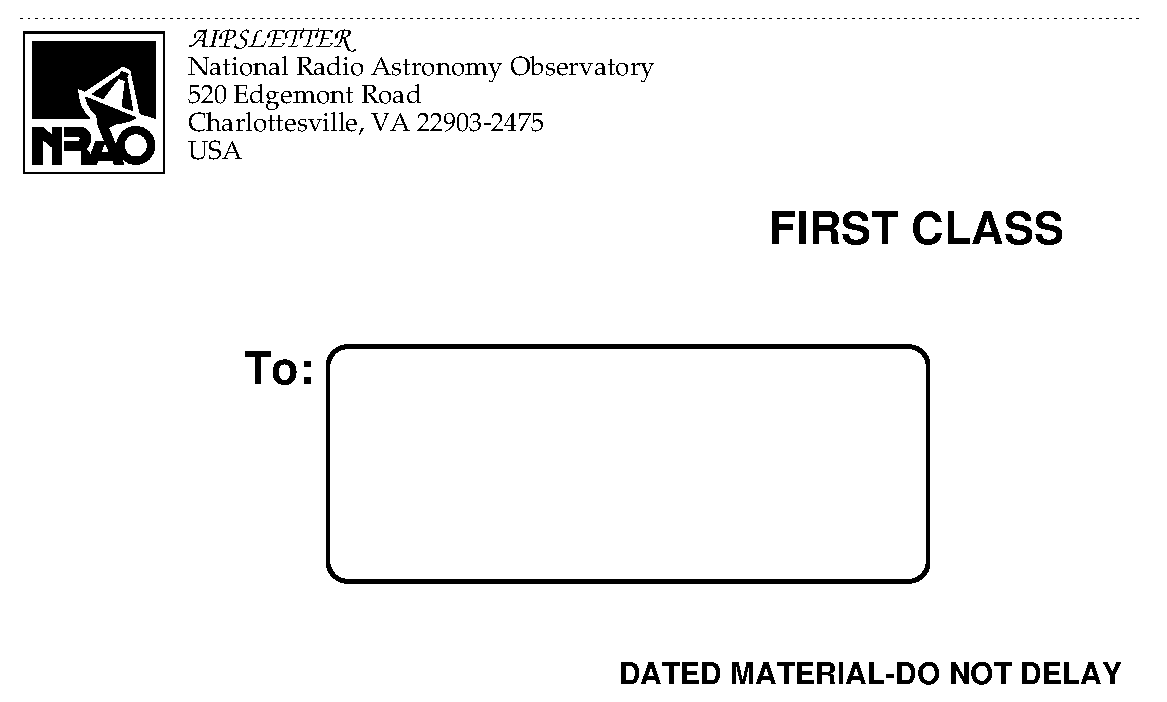
\includegraphics{FIG/AIPSLETM.PS}}}

\end{document}
